\documentclass[a4paper,12pt]{article}
\usepackage{amsmath}
\usepackage{graphicx}
\graphicspath{ {images/} }
\usepackage[utf8]{inputenc}
\usepackage[english]{babel}
\usepackage[document]{ragged2e}
 
\begin{document}\begin{flushleft}\newline \textbf{6.819 PSET 3}
\newline \textbf{09/28/2017}
\end{flushleft}
\newline \begin{center}\textbf{ISAAC KONTOMAH}
\end{center}
\begin{flushleft}
\newline \emph{Collaborators:Devin Morgan , Suman Nepal ,Sanchit Bhatta,Khamoya Ikhofua,Afika Nyati }
\end{flushleft}

\newline \section{Motion Magnification}
\newline \textbf{a.}
\begin{document}
\newline Motion magnification of image A to b 

 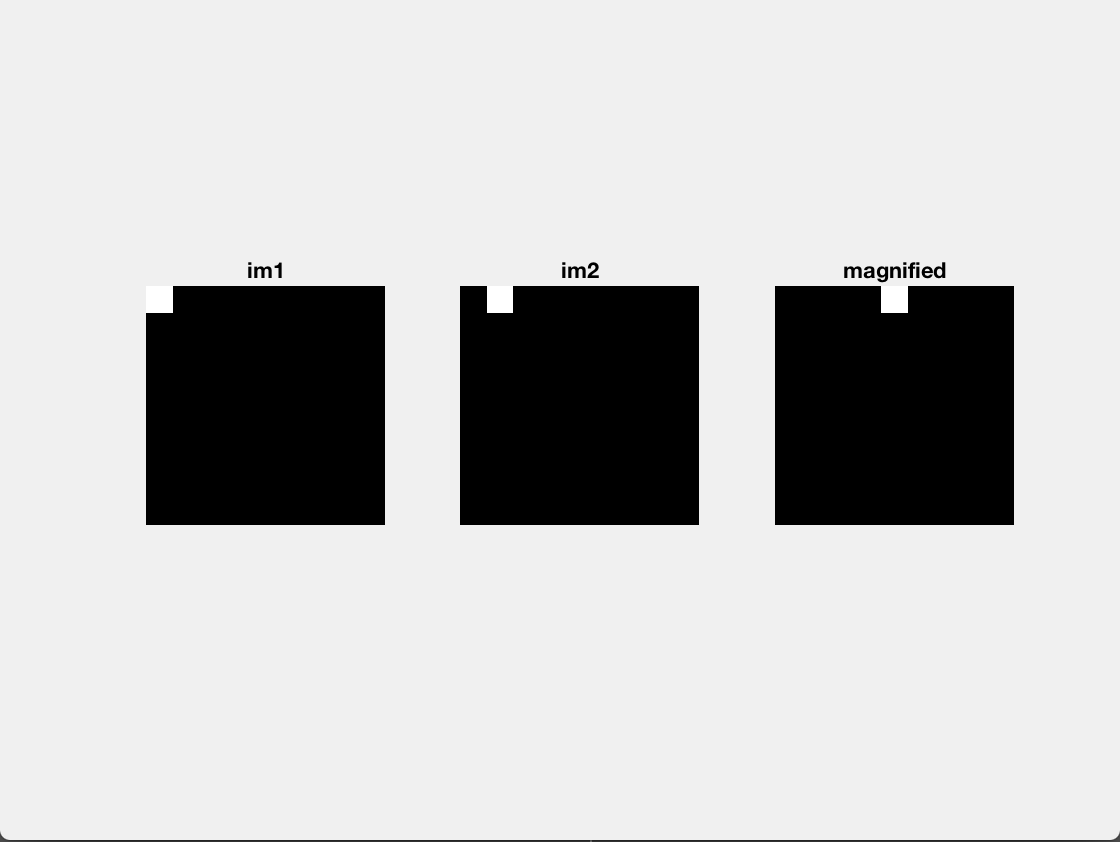
\includegraphics[height=5cm , width=8cm]{magnifychangeA.jpg}

 Image of magnification

\begin{document}
\newline Motion magnification of image A to b 

 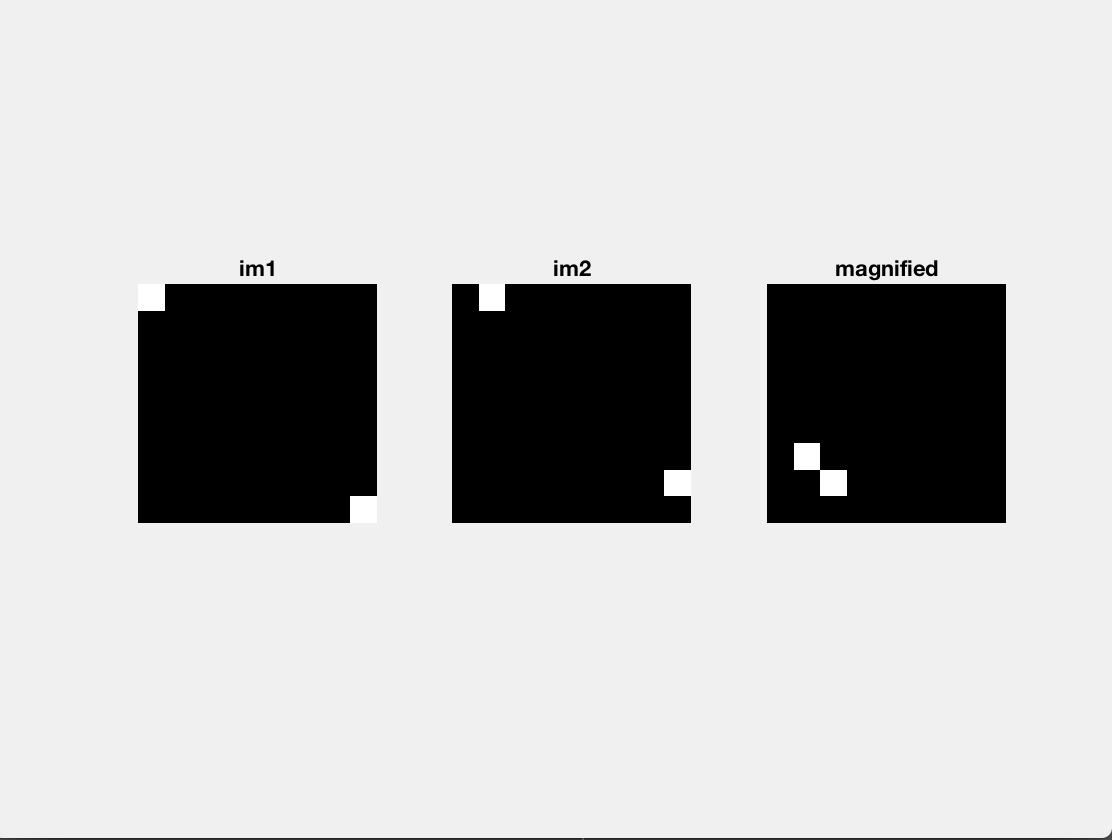
\includegraphics[height=5cm , width=8cm]{magnifychangeB.jpg}

\newline \emph{\textbf{b.Reason offsets are not properly magnified}}
 \newline The phase shift happening in $a$ is been done for one shape while $b$ has 2 boxes hence , the boxes will move to try and find a global phase shift since the phase shift from the magnifyChange function is only applied to one box hence it will have a problem knowing which image to apply the phase shift to
\newline \textbf{c.}
\begin{document}
\newline Gaussian Motion magnification 

 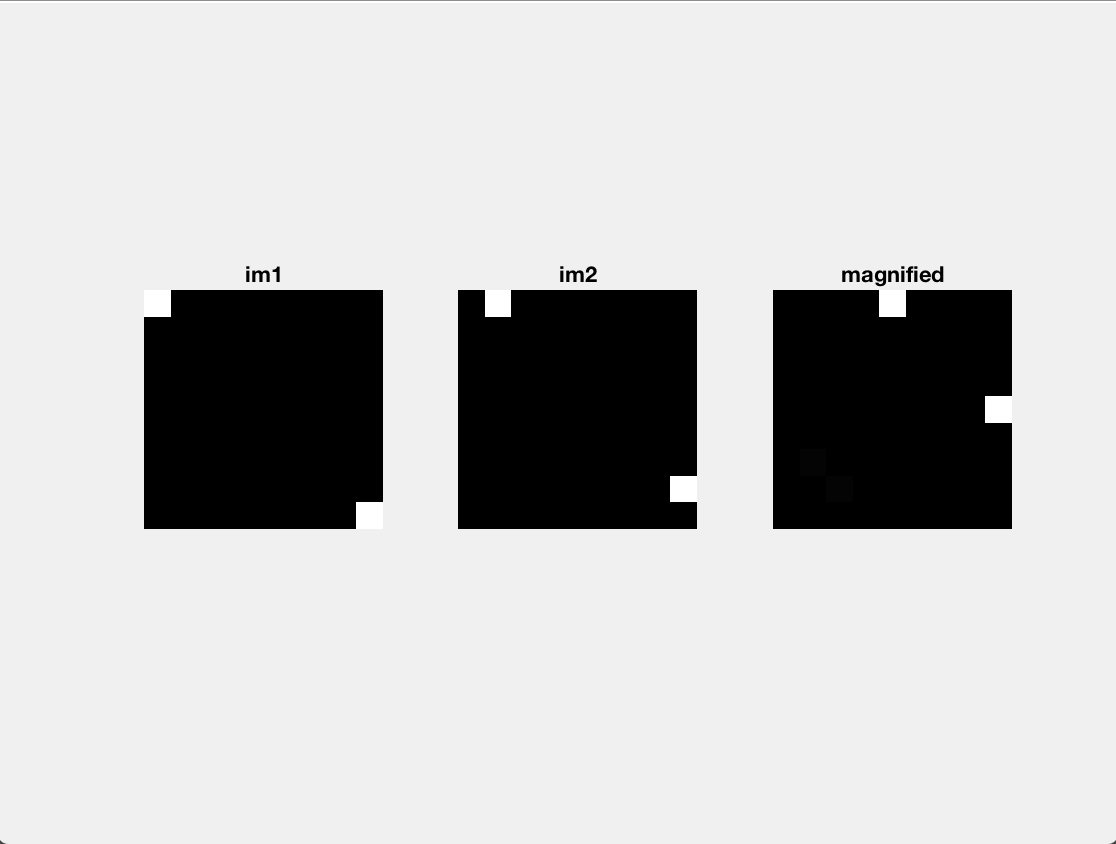
\includegraphics[height=5cm , width=8cm]{magnifychangeC.jpg}

 Image of magnification

\newline \section{Color }
\newline \textbf{a.}
\newline \emph{i.}
\begin{document}
\newline Color spectra

 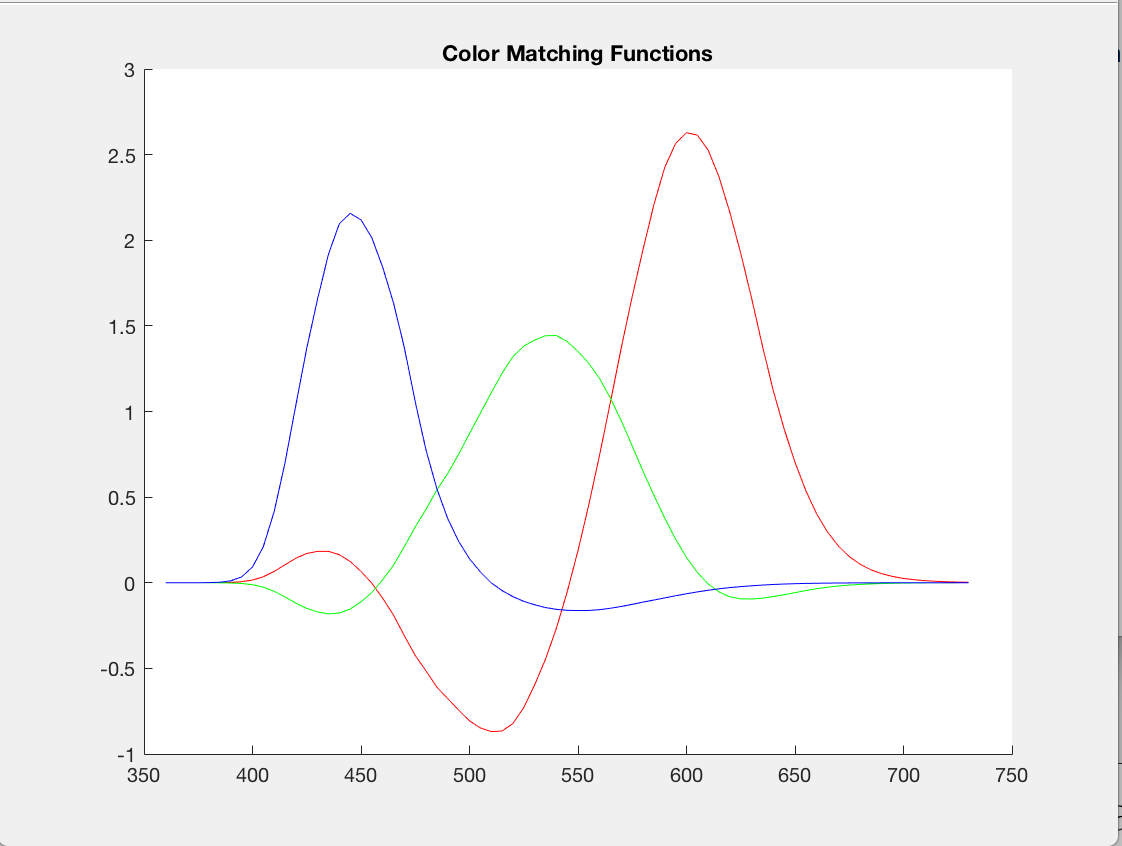
\includegraphics[height=5cm , width=8cm]{colormatchingi.jpg}

 \emph{Positivity : }The blue spectrum is fairly non-negative , the green spectrum is negative between about $400nm$ and $460nm$ and non-negative otherwise , the red spectrum is negative between $450$ and $550nm$ and non-negative otherwise
\newline \emph{ii.}
\begin{document}
\newline Primary Spectra 

 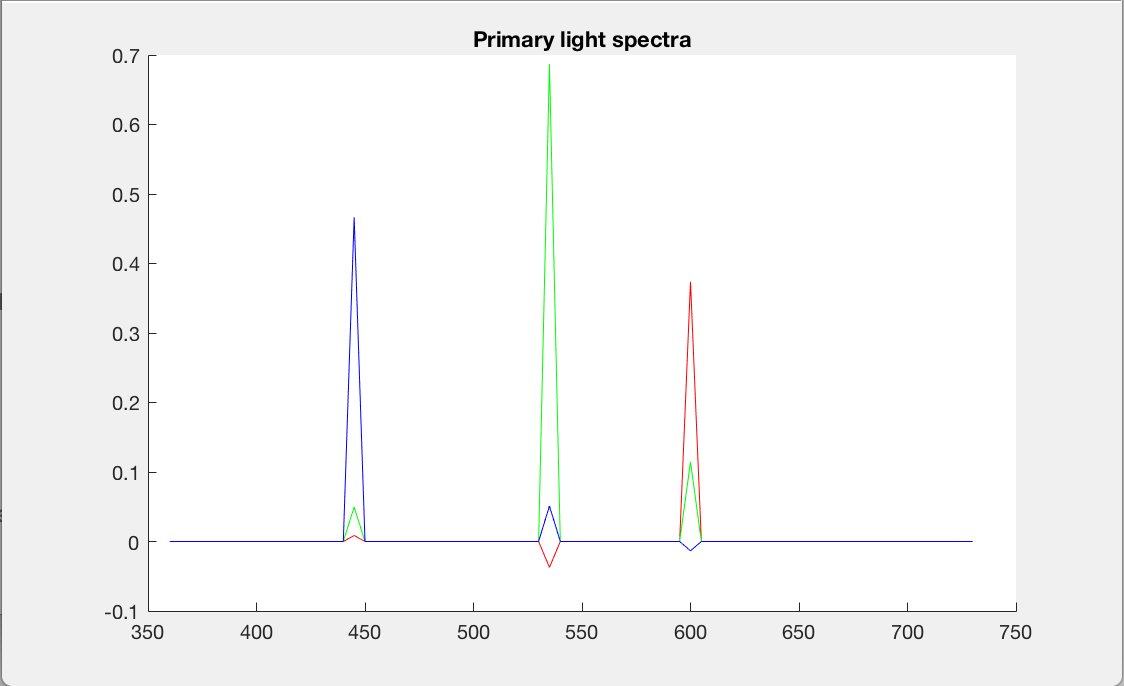
\includegraphics[height=5cm , width=8cm]{primaryspectraII.jpg}

 \emph{Positivity:}At around $440 nm$ , all three are non-negative
 at around $530 nm$, the green and blue primaries are non-negative , the red primary is negative ,at around $600 nm$ ,  the red and green primaries are non-negative,the blue spectra is negative 
\newline \emph{iii.}
\begin{document}
\newline Color Spectra

 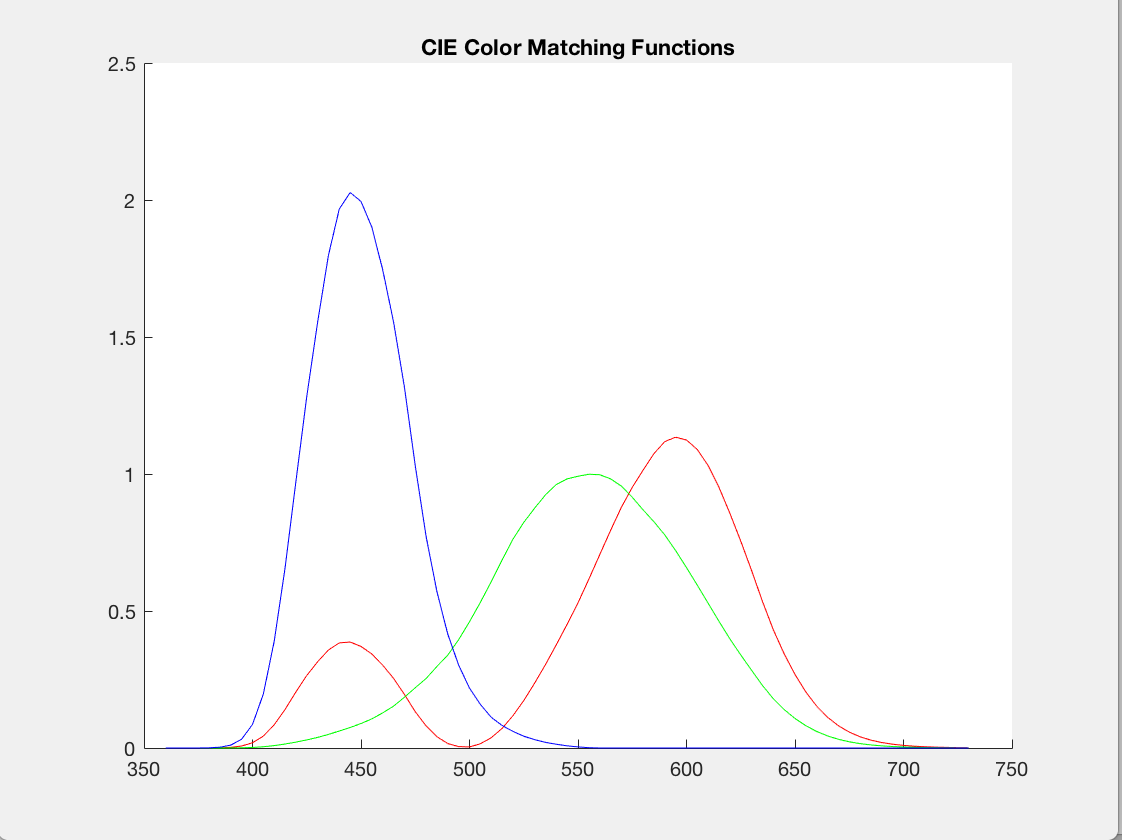
\includegraphics[height=5cm , width=8cm]{ciecolormatchingIII.jpg}

 \emph{Positivity:} All three spectra are non-negative
\newline \emph{iv.}
\begin{document}
\newline Primary spectra

 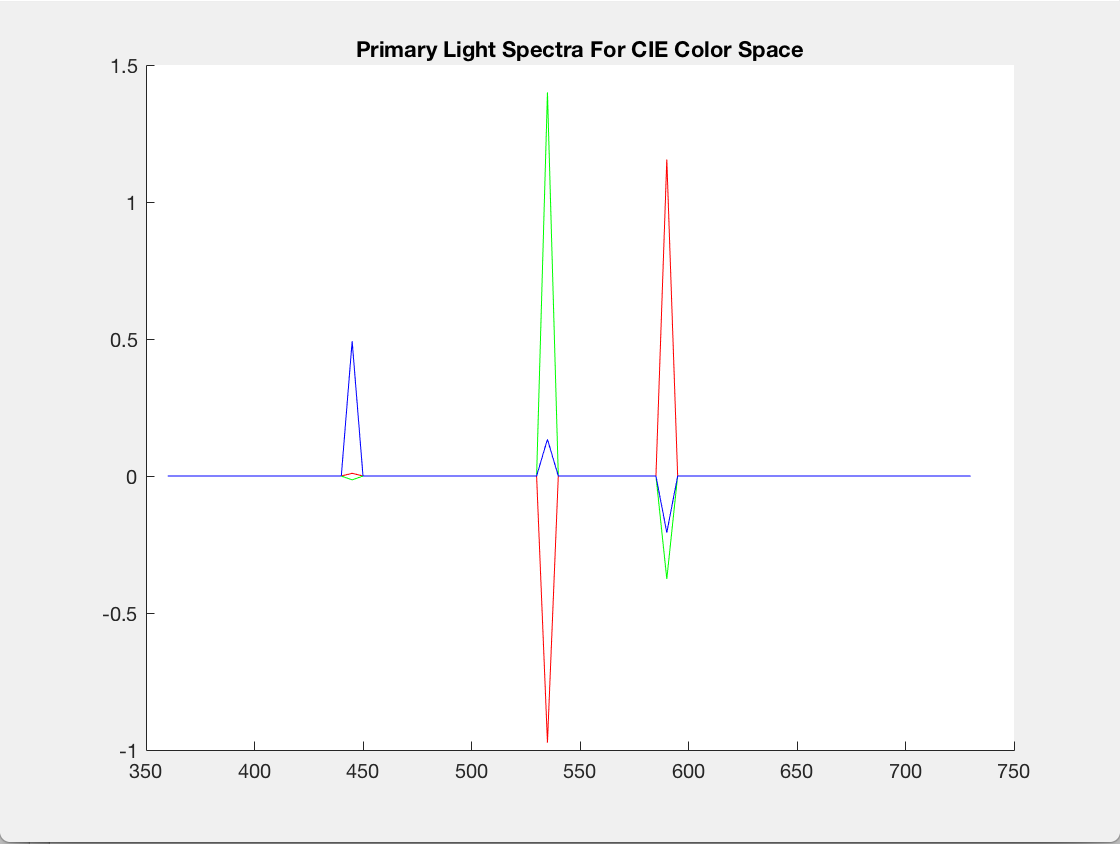
\includegraphics[height=5cm , width=8cm]{primarylightspectraCIE.jpg}

 \emph{Positivity:} At around $440 nm$ , blue and red are non-negative,green is negative
 at around $530 nm$, the green and blue primaries are non-negative , the red primary is negative ,at around $600 nm$ ,  the red primary is non-negative,the blue and green spectra are negative 
\newline \textbf{b.}
\begin{document}
\newline LMS Response Spectra

 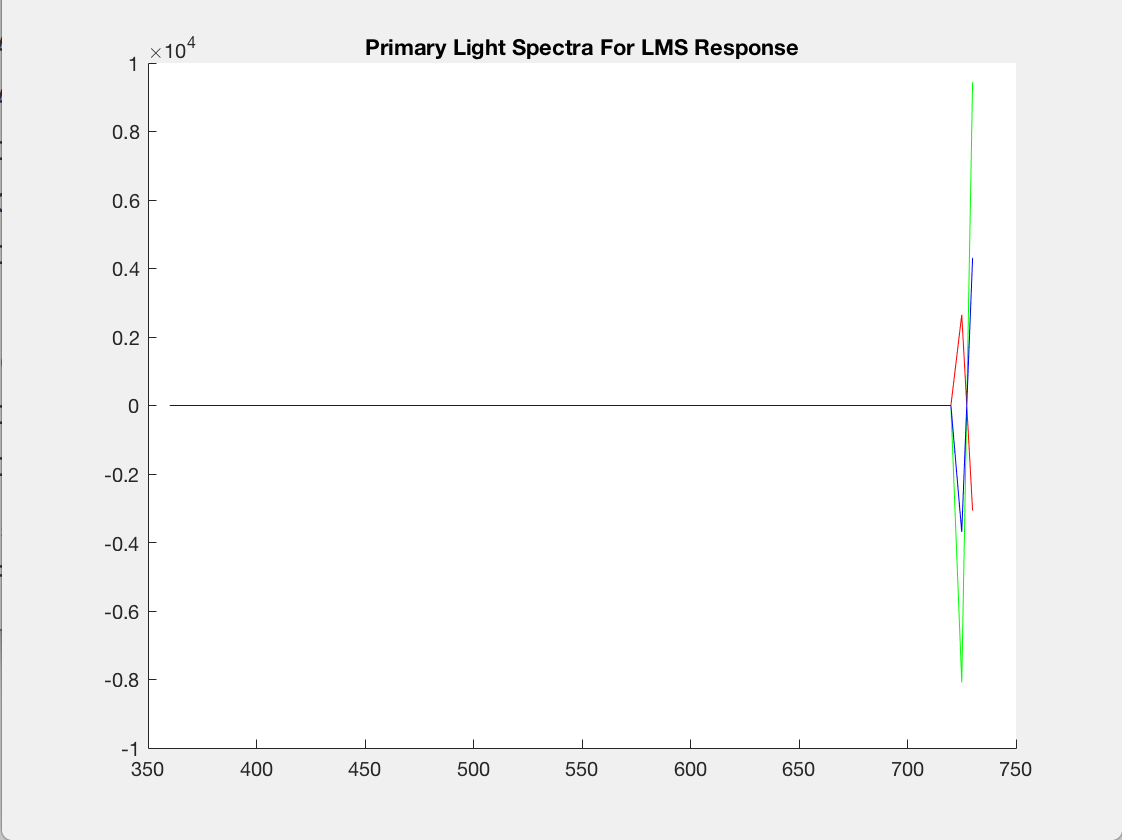
\includegraphics[height=5cm , width=8cm]{lmsresponseprimary.jpg}

 \emph{Positivity:}All three spectra are both negative and positive ie.they have negative and positive components
\newline \textbf{c.}
\newline $C.P=I$
\newline $C=\left[ {\begin{array}{c}
   L^{T}\\
    M^{T} \\
   S^{T}\\
  \end{array} } \right] =\left[ {\begin{array}{ccccc}
   A_{0} & A_{1}& ...&...&A_{n}\\
   B_{0} & B_{1}& ...&...&B_{n}\\
   C_{0} & C_{1}& ...&...&C_{n} \\
  \end{array} } \right] P=\left[ {\begin{array}{ccc}
   p_{11}& p_{12}& p_{13}\\
   p_{21}& p_{22}& p_{23}\\
  p_{31}& p_{32}& p_{33} \\
    ...& ...& ... \\
     ...}& ...& ...\\
      p_{n1}& p_{n2}& p_{n3} \\
  \end{array} } \right]$
  
  \newline $dim(C)= 3 \times n$ , $dim(P)=n \times 3 $ , hence $dim(I)= 3 \times 3$
  \newline $C.P=I=\left[ {\begin{array}{ccc}
   Ap_{1} & Ap_{2}&Ap_{3}\\
    Bp_{1} & Bp_{2}&Bp_{3}\\
  	 Cp_{1} & Cp_{2}&Cp_{3}\\
  \end{array} } \right]=\left[ {\begin{array}{ccc}
   1 & 0& 0 \\
   0& 1& 0\\
   0& 0& 1\\
  \end{array} } \right]$
  \newline $Ap_{1}=1 , Ap_{2}=0 , Ap_{3}=0 \implies A=\frac{1}{p_{1}}=\frac{p_{1}}{||p_{1}||^{2}} \geq 0$ 
  \newline $Bp_{1}=0 , Bp_{2}=1 , Bp_{3}=0 \implies B=\frac{1}{p_{2}}=\frac{p_{2}}{||p_{2}||^{2}} \geq 0$ 
   \newline $Cp_{1}=0 , Cp_{2}=0 , Cp_{3}=1 \implies C=\frac{1}{p_{3}}=\frac{p_{3}}{||p_{3}||^{2}} \geq 0$ 
\end{document}